\section{Définition du cadre du projet}

\subsection{Analyse Benchmark}

\tab L'état de l'art de la détection d'obstacle est actuellement centrée sur les algorithmes dits de SLAM pour \textit{Simultaneous Localization and Mapping}\cite{slam-nexter}. Ces algorithmes sont extrêmement bien adaptés à l'utilisation d'un LiDAR sur un robot possédant d'autres capteurs de déplacements (les encodeurs rotatif incrémentaux sur les roues par exemple), car la fusion de ces capteurs avec les données du LiDAR permet de minimiser les imprécisions de mesure tout en gérant une carte dynamique de l'environnement. Cela permet de surcroît de positionner le robot lui-même dans son environnement. On corrige ainsi les décalages éventuels du robot et de ses encodeurs rotatifs. Plusieurs grandes phases sont discernables dans ce type d'algorithme :

\begin{enumerate}
    \item la récupération des données et le filtrage des données aberrantes,
    \item la recherche d'éléments reconnaissables (point de repères ou \textit{landmarks} dans la littérature),
    \item mise en lien des point de repères entre plusieurs mesures (association, détermination des mouvements),
    \item utilisation de ces point de repères, de la position supposée du robot par ses autres capteurs et de ses positions et cartographies précédentes pour construire la prochaine carte la plus probable.
\end{enumerate}

Actuellement, un très grand travail de recherche est effectué dans le domaine de l'automobile, entre autres, avec l'émergence des véhicules autonomes qui ont besoin d'acquérir énormément de données sur leur environnement. Des systèmes basés sur des LiDARs multicouches (fournissant des nuages de points en 3D et non en 2D comme le nôtre) permettent à ces véhicules de se repérer, éviter les obstacles et suivre la route sans danger.

\subsection{Prise en main du LiDAR}
\subsubsection{Installation}
\tab De nombreux documents et un logiciel de prise en main sont fournis par le constructeur, et les fournisseurs. Vous pourrez trouver entre autres la documentation officielle et un logiciel d’affichage de données en temps réel sur le lien suivant :\newline \href{https://www.robotshop.com/en/rplidar-a2-360-laser-scanner.html}{\textit{Lien vers le site robotshop.}}\footnote{https://www.robotshop.com/en/rplidar-a2-360-laser-scanner.html}

\begin{figure}[htp]
    \centering
    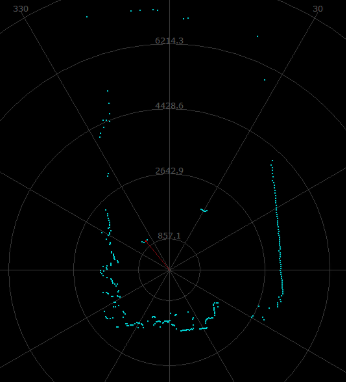
\includegraphics[width=6cm]{/Cadre/demo.PNG}
    \caption{Logiciel de démonstration du capteur fourni.}
\end{figure}

Pour nos premiers tests, nous avons utilisé une bibliothèque existante en Python permettant une prise en main rapide et sûre du lidar, avec des gestions de cas d’erreurs et de validité de données envoyées par le lidar.
\href{https://github.com/Roboticia/RPLidar}{\textit{Lien vers la bibliothèque.}}\footnote{https://github.com/Roboticia/RPLidar}


Nous avons également réalisé une plateforme de test fixe pour maîtriser le capteur avant de l’embarquer dans un robot:

\begin{figure}[htp]
    \centering
    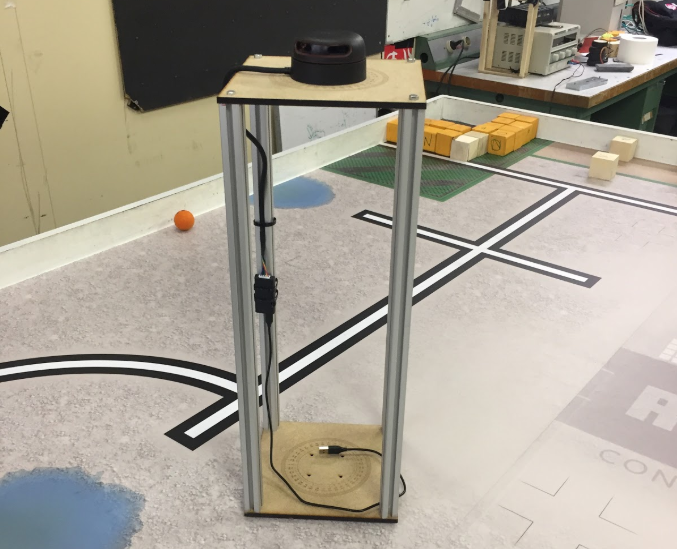
\includegraphics[width=6cm]{/Cadre/plateforme_test.PNG}
    \caption{Plateforme de test.}
\end{figure}

\subsubsection{Étude de la fiabilité du LiDAR}
\paragraph{Étude des valeurs aberrantes}
\tab Lors de nos premières phases de tests, nous avons pu observer la présence de valeurs aberrantes dans nos mesures, allant parfois jusqu'à plusieurs centimètres d'écart à la réalité. Mais la majorité des valeurs étant à quelques millimètres d'écarts, un filtrage simple doit permettre de retirer ces aberrations.
On remarque en outre une grande importance du choix de la vitesse en rotation, ces aberrations étant plus présentes à basses ou hautes vitesses, mais moins en vitesses moyennes, proches de celle par défaut à 10Hz.

\begin{figure}[htp]
    \centering
    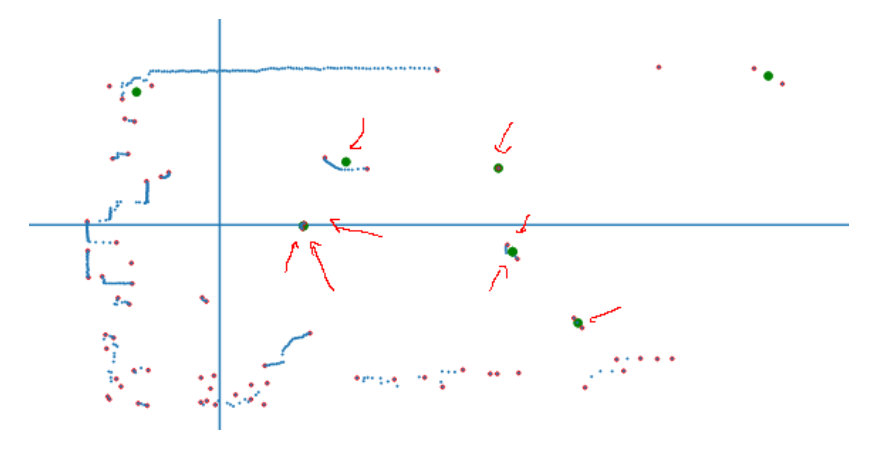
\includegraphics[width=6cm]{/Cadre/premier_test.PNG}
    \caption{Visuel du premier test réalisé avec le LiDAR.}
\end{figure}

\tab Par rapport à la documentation, on remarque également que la vitesse maximale réelle est 19Hz et pas 15Hz comme indiqué, mais nous resterons dans les standards (valeur conseillée étant de 60\% du PWM maximal, correspondant à une fréquence de mesure 10Hz) pour éviter d'user le composant et éviter d'endommager notre terminal, le port USB ne pouvant fournir qu'un courant limité dans le cas où l'alimentation du LiDAR se ferait uniquement par l'USB.

\paragraph{Choix d'une vitesse de rotation}

\tab Afin de déterminer une vitesse de rotation, nous avons procédé de la façon suivante :
Nous prenons des mesures sur 20 secondes. Pour un angle donné, on récupère les valeurs qui sont compris dans [Angle-0.5,Angle+0.49]. On trace alors un graphe pour chaque vitesse.

\tab On remarque alors qu'une vitesse basse donne des mesures plus dispersées et qu'un vitesse très élevée donne souvent un résultat proche de la réalité mais donne parfois un résultat biaisé.

\tab $ V \simeq 500$ (Ce qui correspond à un PWM à 48.8\%) semble être la vitesse idéale, ce PWM offrant une vitesse moyenne. On obtient alors une distribution relativement gaussienne, ce qui est plus adapté à un traitement par filtre de Kalman par exemple.

%image angle et vitesse

\paragraph{Choix d'une résolution angulaire}
\tab On estime que la distance utile, c'est à dire la distance maximale pour laquelle on estime qu'il faut détecter les obstacles est de 3m.
On estime également qu'il faudrait avoir une précision d'au moins 2,5cm à 3cm.

% Comment arrive-t-on jusqu'ici ?
\tab Pour cela on doit avoir 0.5 degré de résolution, On réalise alors une discrétisation angulaire à 0,5 degré près. 

% Expliciter le raisonnement et rajouter un schéma
\paragraph{Choix du nombre de scans avant traitement}
\tab Nous voulions dans un premier temps trouver un nombre de scans (c'est à dire le nombre de tour de mesure) avant traitement afin d'essayer d'avoir une valeur pour chaque angle selon notre résolution angulaire. Dans l'idée de départ, nous imaginions un système avec un temps de mesure + traitement inférieur 1,5 seconde.

\tab Le LiDAR réalisant 10 scans par seconde à la vitesse $V = 500 $, nous pouvions envisager une valeur de scans avant traitement entre 1 et 10. Tous les paramètres de mesure sont regroupés dans le projet final dans un fichier de configuration qui nous permet de jouer comme sur ces paramètres facilement comme on le souhaite. Les essais nous ont montré que finalement il était plus efficace et précis de faire un traitement après chaque scan. En effet, même si nous avons pas une valeur pour chaque angle, nous réduisons le traitement à réaliser en s'affranchissant de calculs de moyenne par exemple si nous avons plusieurs valeurs pour un angle donné en réalisant plusieurs tours. On remarque en effet la formation de traînées derrière les objets en mouvement, ce qui était causé par ces moyennes sur N tours. Le traitement sur un tour nous affranchit de ce problème.